%%%%%%%%%%%%%%%%%%%%%%%%%%%%%%%%%%%%%%%%%
% Beamer Presentation
% LaTeX Template
% Version 1.0 (10/11/12)
%
% This template has been downloaded from:
% http://www.LaTeXTemplates.com
%
% License:
% CC BY-NC-SA 3.0 (http://creativecommons.org/licenses/by-nc-sa/3.0/)
%
%%%%%%%%%%%%%%%%%%%%%%%%%%%%%%%%%%%%%%%%%

%----------------------------------------------------------------------------------------
%	PACKAGES AND THEMES
%----------------------------------------------------------------------------------------

\documentclass{beamer}

\mode<presentation> {

% The Beamer class comes with a number of default slide themes
% which change the colors and layouts of slides. Below this is a list
% of all the themes, uncomment each in turn to see what they look like.

%\usetheme{default}
%\usetheme{AnnArbor}
%\usetheme{Antibes}
%\usetheme{Bergen}
%\usetheme{Berkeley}
%\usetheme{Berlin}
%\usetheme{Boadilla}
%\usetheme{CambridgeUS}
%\usetheme{Copenhagen}
%\usetheme{Darmstadt}
%\usetheme{Dresden}
%\usetheme{Frankfurt}
%\usetheme{Goettingen}
%\usetheme{Hannover}
%\usetheme{Ilmenau}
%\usetheme{JuanLesPins}
%\usetheme{Luebeck}
\usetheme{Madrid}
%\usetheme{Malmoe}
%\usetheme{Marburg}
%\usetheme{Montpellier}
%\usetheme{PaloAlto}
%\usetheme{Pittsburgh}
%\usetheme{Rochester}
%\usetheme{Singapore}
%\usetheme{Szeged}
%\usetheme{Warsaw}

% As well as themes, the Beamer class has a number of color themes
% for any slide theme. Uncomment each of these in turn to see how it
% changes the colors of your current slide theme.

%\usecolortheme{albatross}
%\usecolortheme{beaver}
%\usecolortheme{beetle}
%\usecolortheme{crane}
%\usecolortheme{dolphin}
%\usecolortheme{dove}
%\usecolortheme{fly}
%\usecolortheme{lily}
%\usecolortheme{orchid}
%\usecolortheme{rose}
%\usecolortheme{seagull}
%\usecolortheme{seahorse}
%\usecolortheme{whale}
%\usecolortheme{wolverine}

%\setbeamertemplate{footline} % To remove the footer line in all slides uncomment this line
%\setbeamertemplate{footline}[page number] % To replace the footer line in all slides with a simple slide count uncomment this line

%\setbeamertemplate{navigation symbols}{} % To remove the navigation symbols from the bottom of all slides uncomment this line
}

\usepackage{graphicx} % Allows including images
\usepackage{booktabs} % Allows the use of \toprule, \midrule and \bottomrule in tables
\usepackage{amsmath}
\graphicspath{{talk_images/}}

%----------------------------------------------------------------------------------------
%	TITLE PAGE
%----------------------------------------------------------------------------------------

\title[ACM ICPC Boot Camp]{ACM ICPC Boot Camp} % The short title appears at the bottom of every slide, the full title is only on the title page
\author{Ankesh Gupta}
\institute[IITD]
{
IIT Delhi \\ % Your institution for the title page
Credits: Adapted from IIT Bombay Slides
}
% \email{ankeshgupta007@gmail.com}% 
% \author{Adapted from IIT Bombay Slides}
\date{\today} % Date, can be changed to a custom date

\begin{document}

\begin{frame}
\titlepage % Print the title page as the first slide
\end{frame}


\begin{frame}
\frametitle{What is ACM ICPC?}
\begin{itemize}
\item ICPC stands for Inter-Collegiate Programming Contest,
conducted by ACM
\item It is the most prestigious college level programming contest
\item 3 stages - Online, Onsite(regionals), World Finals
\item Online round has ~3500 teams participating
\item India conducts 4-5 regionals(this year 4)
\end{itemize}
\end{frame}

%------------------------------------------------

\begin{frame}
	\begin{figure}[!htb]
		\centering
		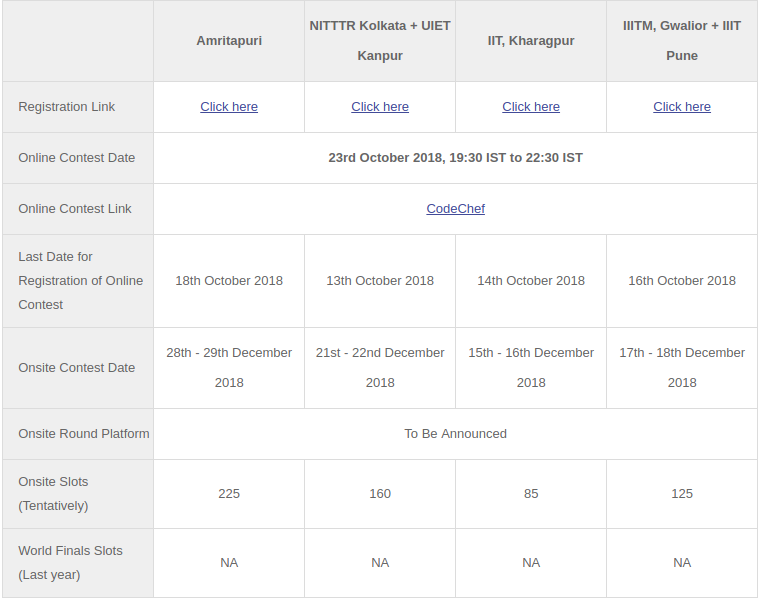
\includegraphics[width=0.8\textwidth]{this_year_stats.png}
	\end{figure}
\end{frame}

\begin{frame}
\frametitle{How to Participate?}
\begin{itemize}

\item Teams of 3.
\item Each team should have a coach, who must be a professor.
\item The coach registers the team for the online round.
\item Typically 2-3 teams qualify from the institute per regional after online round.
\item Preference given to maximise number of distinct colleges at a regional.
% \item Registration has already started. Check previous slides for details.
\end{itemize}
\end{frame}

%------------------------------------------------

\begin{frame}
\frametitle{A Typical Contest Problem}
\begin{itemize}

\item Problem
\item Input and Output format
\item Number of instances
\item Variable bounds
\item Constraints
\begin{itemize}
\item Time limit
\item Space limit
\end{itemize}
\end{itemize}
\end{frame}

%------------------------------------------------

\begin{frame}
\frametitle{Input/Output Format}
\begin{itemize}
\item Input is from STDIN and output is to be made to STDOUT
\item For C++: scanf and printf are in general faster than cin and cout, so it is recommended that you use these for i/o handling.
\item General Tip: Time for i/o depends on the number of system calls made, so for instance if you have to take as input 'n' numbers, separated by space, it is useful to take the input as a single line and then parse it to get 'n' numbers rather than making 'n' different system calls.
\item Make sure that you follow the output format and avoid trivial wrong submissions only because of formatting the output incorrectly.
\end{itemize}
\end{frame}

%------------------------------------------------
\section{Second Section}
%------------------------------------------------

\begin{frame}
\frametitle{O-notation}
\begin{itemize}
\item O-notation : \newline
f(n) = O(g(n)) if f (n) is asymptotically less than some
multiple of g(n).
\item Generally helpful to estimate complexity of algorithms.
\item For example,

$f(n) = 2n^2 + 4n^3 = O(n^3)$
\end{itemize}
\end{frame}

%------------------------------------------------

\begin{frame}
\frametitle{Variable Bounds}
\begin{itemize}
\item A typical CPU is assumed to process $10^8$ instructions in a second.
\item This assumption will help us deciding the targetted order of the algorithm while inspecting the input variable constraints.
\item A brief idea is as follows:
Divide $10^8$ by the number of test cases and then use the following table to predict order.

\begin{table}
\begin{tabular}{l l}
\toprule
\textbf{Variable Bound * No. Test Cases} & \textbf{Predicted Order}\\
\midrule
$10^8$ & O(n)\\
$10^5$ & O(nlogn)\\
$10^4$ & O($n^2$)\\
$10^{16}$ & O($\sqrt{n}$),O(nlogn)\\
\bottomrule
\end{tabular}
\end{table}


\end{itemize}
\end{frame}

%------------------------------------------------
\begin{frame}
\frametitle{Data Ranges}
\begin{itemize}
\item It is important that you understand which data type to use.
\item For this it is necessary to have a feel of the ranges of various data types.
\item This avoids loss of time during the competition in figuring out the appropriate data type say long int or just int or long long int.

\item The foll. table gives a brief idea about some data types. You can google for other data types.
%------------------------------------------------

\begin{table}
\begin{tabular}{l l}
\toprule
\textbf{Data Type} & \textbf{Range}\\
\midrule
short & –32,768 to 32,767\\
int &  –2,147,483,648 to 2,147,483,647\\
long long  & –9,223,372,036,854,775,808 - 9,223,372,036,854,775,807\\
\bottomrule
\end{tabular}
\end{table}
\end{itemize}
\end{frame}

%------------------------------------------------

\begin{frame}
\frametitle{Types of errors}
\begin{itemize}
\item Compilation Error
\item Time Limit Exceeded
\item Memory Limit Exceeded
\item Wrong Answer
\item You should be familiar with these errors before attempting a contest
\item Appropriate penalties are put for every erroneous solution
\end{itemize}
\end{frame}


%------------------------------------------------

\begin{frame}
\frametitle{Programming Style}
\begin{itemize}
\item C, C++, Java is allowed in all contests. So preferably practice
in only these
\item Using templates can ease your job during a contest
\item Be aware! Corner cases can get tricky!
\item Be careful about the output format; take care in removing
stray outputs.
\end{itemize}
\end{frame}

%------------------------------------------------

%------------------------------------------------

\begin{frame}
\frametitle{C++ Standard Template Library}
\begin{itemize}
\item Using STL classes/functions can speed up your work.
\item They may be more efficient than your own implementation.
\item Some STL classes that help, \newline
vector, list, queue, set, map, deque, priority queue
\item STL functions that help, \newline
sort, next permutation, etc...
\end{itemize}
\end{frame}

%------------------------------------------------
\begin{frame}
\frametitle{C++ Algorithms Library}
\begin{itemize}
\item Algorithms library is a very important library with many predefined functions which can be used directly and inturn save time.
\item Some important functions are:
\begin{itemize}
\item Merge
\item Sort
\item Min/Max
\item Lexographical Compare
\item Make Binary Heap
\item Modifying/Nonmodifying Sequence Operations
\end{itemize}
\end{itemize}
\end{frame}

%------------------------------------------------



%------------------------------------------------

\begin{frame}
\frametitle{Where and How to Practice?}
\begin{itemize}
\item Codeforces div3, div2, educational rounds, div1
\item Codechef cookoff (monthly contest) and long contests should be tried
\item SPOJ solutions are not easy to find but lots of discussion available online for same
\item Hackerearth, Hackerrank - simple platform with a good interface and problems escalating from simple to difficult
\end{itemize}
\end{frame}

%------------------------------------------------
\begin{frame}
\frametitle{Success is team work}
\begin{itemize}
\item Knowing who does what best can help in planning
\item Try forming a team with people having different strengths
\item Cross check your teammate’s solution for higher accuracy before submitting
\item Ensure that all three are not stuck on the same problem. Start attacking different problems
\item Stay cool! Don’t panic! :)
\end{itemize}
\end{frame}

%------------------------------------------------

%------------------------------------------------

\begin{frame}
\Huge{\centerline{Thank You!}}
\end{frame}

%----------------------------------------------------------------------------------------

\end{document}